\subsection{Mikroprocessor}
\subsubsection{Arduino Mega 2560}
Som alternativ til at anvende UCN boardet, er et Arduino Mega 2560 board blevet brugt. Dette er gjort da der i videreudvikling benyttes shields som ikke er kompatibel med UCN boardet. Endvidere skal der bruges mere hukommelse til videreudviklingen, end UCN boardet har til rådighed.
\\
\\
Mikroprocessoren besidder 54 digitale pins og 14 analog pins der fungerer som in- og output. Derudover har den 4 UART(Universal asynchronous receiver/transmitter) pins som anvedes til at integrere med microproicessorens interface.
\\
\\
Disse pins fungerer i spændingsintervallet mellem 0-5 V. ATMega2560 er Arduino Mega's processor og har en clock frekvens på 16 MHz. Strømmen tilføres gennem usb, power jack eller gennem pin $V_{in}$ og anbefales en spænding mellem 7-12 V. 
\\
\\
Mikroprocessoren kan forbindes til computeren ved hjælp af usb, som gør det muligt for de to enheder at kommunikere sammen. Gennem usb forbindelsen kan softwaren overføres fra computeren til den anden enhed. Om nødvendigt kan softwaren genstartes på mikroprocessoren gennem en resetknap, som er monteret på dens PCB(Printed Circuit Board).
\newline 
Arduino Mega 2560 har den fordel at være kombatibel med standard bibliotekerne fra Arduino, hvorimod UCN boardet vil kræve at alt softwaren skal bygges fra begyndelsen.

\begin{figure}[h!]
  \centering
  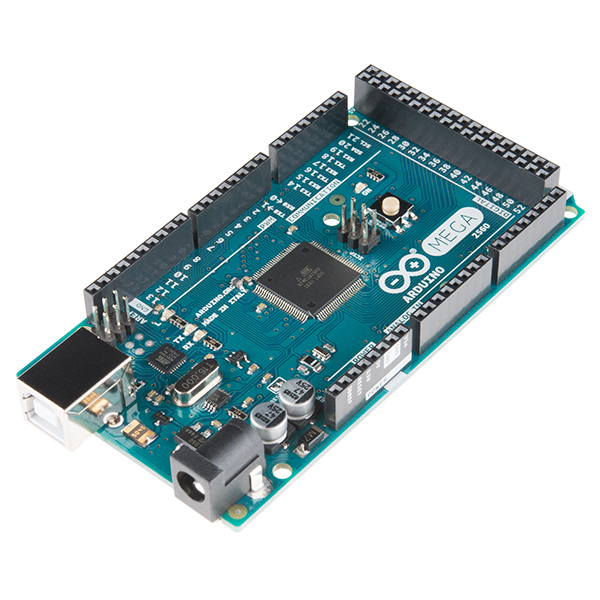
\includegraphics[width=0.7\textwidth]{figures/arduinoMega.jpg}
  \caption{Arduino Mega 2560.}
  \label{arduino2569}
\end{figure} 

\newpage



